\documentclass[a4paper,slidestop,xcolor=pst,blue]{beamer}

\input{slidesHeader.tex}

\title[Capa de Persistencia]{Capa de Persistencia}

\author[P. S{\'a}nchez]{\alert{Pablo S{\'a}nchez}}

\institute[IIE]{
		   Dpto. Ingenier{\'i}a Inform{\'a}tica y Electr{\'o}nica \\
		   Universidad de Cantabria \\
		   Santander (Cantabria, Espa{\~n}a) \\
		   \texttt{p.sanchez@unican.es}
}

\date{}

\begin{document}

\begin{frame}[c]
	\titlepage
	\begin{columns}
		\column{0.50\linewidth}
			\centering
    		\includegraphics[width=.28\textwidth,keepaspectratio=true]{images/istr.eps}
		\column{0.50\linewidth}
			\centering
			\includegraphics[width=.25\textwidth,keepaspectratio=true]{images/uc.eps}
	\end{columns}
\end{frame}

\begin{frame}[c]
    \frametitle{\alert{Advertencia}}
    \begin{center}
        Todo el material contenido en este documento no constituye en modo alguno una obra de referencia o apuntes oficiales mediante el cual se puedan preparar las pruebas evaluables necesarias para superar la asignatura. \ \\
        \ \\
        Este documento contiene exclusivamente una serie de diapositivas cuyo objetivo es servir de complemento visual a las actividades realizadas en el aula para la transmisi{\'o}n del contenido sobre el cual versar{\'a}n las mencionadas pruebas evaluables.  \ \\
        \ \\
        Dicho de forma m{\'a}s clara, \alert{estas transparencias no son apuntes y su objetivo no es servir para que el alumno pueda preparar la asignatura.}
    \end{center}
\end{frame}

\section{Introducción}

\subsection{Objetivos y Bibliografía}

\begin{frame}[c]
    \frametitle{Objetivos del Tema}
    \begin{enumerate}[<+->]
         \item Comprender en profundidad cuáles son las responsabilidades de la capa de presentación.
         \item Conocer cómo se relacionan las diferentes tecnologías que integran una capa de presentación web.
         \item Ser capaz de utilizar las etiquetas básicas de HTML.
         \item Conocer los principios y elementos básicos de CSS.
         \item Conocer los principios y elementos básicos del DOM de HTML.
         \item Conocer los principios y elementos básicos de Javascript.
         \item Conocer el objetivo y funcionamiento básico de \emph{bootstrap}.
         \item Comprender el funcionamiento de una llamada AJAX.
         \item Comprender el concepto de componente gráfico.
         \item Comprender los fundamentos del patrón \emph{Single Page Application (SPA)}.
         \item Ser capaz de construir una interfaz SPA utilizando AngularJS.
    \end{enumerate}
\end{frame}

\begin{frame}[c]
    \frametitle{Bibliografía}
    \begin{thebibliography}{1}

        \bibitem[Esposito and Saltarello, 2014]{Esposito2014}
        Esposito, D. y Saltarello, A. (2014).
        \newblock {\em {Microsoft .NET - Architecting Applications for the
          Enterprise}}. 2ª Ed..
        \newblock Microsoft Press

        %% SPA

        %% AngularJS

        %% HTML

        %% CSS

        %% Javascript

        %% AJAX

    \end{thebibliography}
\end{frame}

\subsection{Contexto: Capa de Persistencia}

\begin{frame}
    \frametitle{Capa de Persistencia}
    \only<1|handout:2>{
        \rput[lt](0,0){
            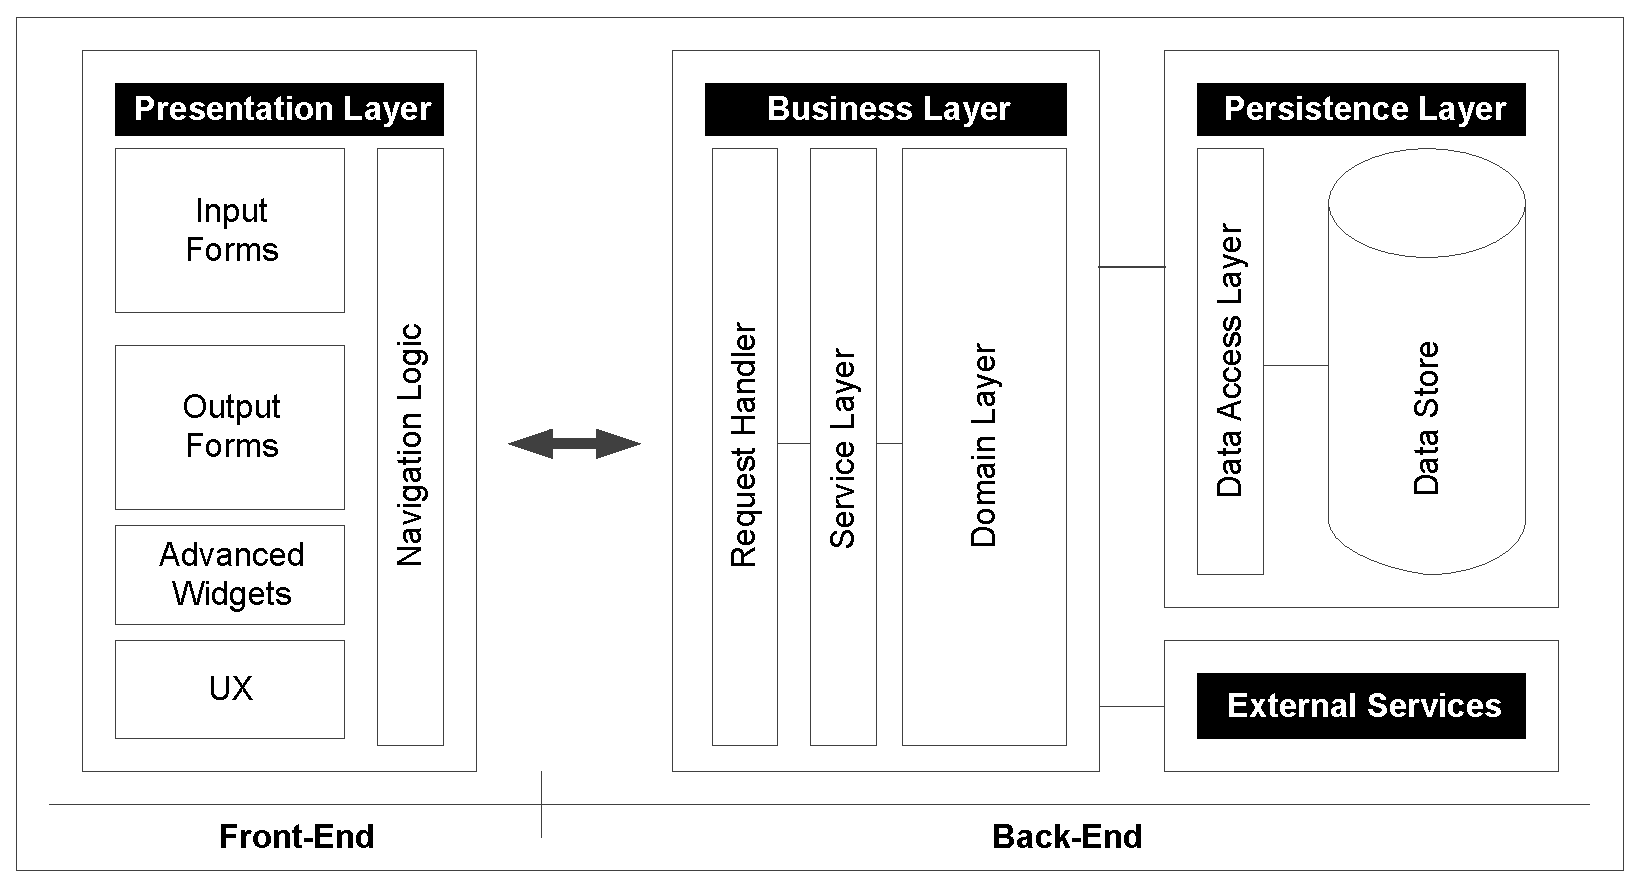
\includegraphics[width=\linewidth]{images/intro/enterpriseArchitectures00.eps}
        }
    }
    \only<2|handout:2>{
        \rput[lt](0,0){
            \includegraphics[width=\linewidth]{images/intro/enterpriseArchitectures01.eps}
        }
    }
\end{frame}

\subsection{Tecnologías de la Capa de Persistencia}

\begin{frame}[c]
	\frametitle{Responsabilidades de la Capa de Presentación}
	\begin{enumerate}[<+->]
        \item Permitir a los usuarios interactuar con el sistema.
        \item Introducir datos en el sistema (validándolos previamente).
        \item Visualizar los datos de manera amigable al usuario.
        \item Facilitar operaciones simples (filtros y redistribuciones) sobre los datos.
        \item Facilitar la navegación por el sistema.
        \item Mejorar la experiencia de usuario (UX). %% Hellmans
        \item Mantener la comunicación con el servidor.
        \item Gestionar situaciones excepcionales.
	\end{enumerate}
\end{frame}

\begin{frame}[c]
    \frametitle{Tecnologías de una Capa de Presentación Web}
    %% Meter Imagen
\end{frame}

\section{HTML}

\begin{frame}[c]
    \frametitle{HTML}
    %% Definición
\end{frame}

\begin{frame}[c]
    \frametitle{Head y Body}
    %% Definición
\end{frame}

\begin{frame}[c]
    \frametitle{Directivas Cabecera}
    %% Definición
\end{frame}


\begin{frame}[c]
    \frametitle{HTML - Etiquetas Básicas}
    \begin{description}
        \item[p]
        \item[h1-5]
        \item[img]
        \item[a]
        \item[br]
    \end{description}
\end{frame}

\begin{frame}[c]
    \frametitle{HTML - Formateo de Fuentes}
    \begin{description}
        \item[em]
        \item[strong]
        \item[mark]
        \item[sub]
        \item[sup]
    \end{description}
\end{frame}

\begin{frame}[c]
    \frametitle{HTML - Listas}
    \begin{description}
        \item[ol]
        \item[ul]
        \item[dl]
        \item[li]
    \end{description}
\end{frame}

\begin{frame}[c]
    \frametitle{HTML - Tablas}
    \begin{description}
        \item[table]
        \item[tr]
        \item[td]
        \item[th]
    \end{description}
\end{frame}

\begin{frame}[c]
    \frametitle{HTML - Maquetación Básica}
    \begin{description}
        \item[div]
        \item[span]
    \end{description}
\end{frame}

\begin{frame}[c]
    \frametitle{HTML - Maquetación Avanzada}
    %% Hacer imagen
    \begin{description}
        \item[header]
        \item[nav]
        \item[section]
        \item[article]
        \item[aside]
        \item[footer]
    \end{description}
\end{frame}

\section{CSS}

\begin{frame}[c]
    \frametitle{CSS}
    %% Definición
\end{frame}

\begin{frame}[c]
    \frametitle{CSS - Inclusión en HTML}
    %% Formas de enlazado
    %% Incrustado en un elemento.
    %% Interno en HTML
    %% Fichero externo
\end{frame}

\begin{frame}[c]
    \frametitle{CSS - Web Adaptativa}
    %% Definición
    %% Web responsiva
\end{frame}

\begin{frame}[c]
    \frametitle{CSS - Viewport}
    %% Definición
    %% Web responsiva
\end{frame}

\begin{frame}[c]
    \frametitle{CSS - Unidades}
    \begin{description}
        \item[cm]
        \item[in]
        \item[px]
        \item[pt]
    \end{description}
\end{frame}

\begin{frame}[c]
    \frametitle{CSS - Unidades}
    \begin{description}
        \item[em]
        \item[rem]
        \item[vh]
        \item[vw]
        \item[vh]
        \item[vw]
    \end{description}
\end{frame}

\begin{frame}[c]
    \frametitle{CSS - Modelo de Cajas}
    %% Imagen
    %% https://www.w3schools.com/css/css_boxmodel.asp
    %% Box-sizing
\end{frame}

\begin{frame}[c]
    \frametitle{CSS - Esquema de una propiedad}
    %% font-family, size, decoration, color
    %% background-color, background-image,
    %% border (style, width, color, collapse),
    %% margin
    %% padding
    %% height, width
\end{frame}

\begin{frame}[c]
    \frametitle{CSS - Propiedades Básicas}
    %% font-family, size, decoration, color
    %% background-color, background-image,
    %% border (style, width, color, collapse),
    %% margin
    %% padding
    %% height, width
\end{frame}

\begin{frame}[c]
    \frametitle{CSS - Reglas}
    %% Selector, propueddes
\end{frame}


\begin{frame}[c]
    \frametitle{CSS - Selectores}
    %% Elemento
    %% Clase
    %% Id
    %% Anidamiento
\end{frame}

\begin{frame}[c]
    \frametitle{CSS - Pseudoselectores}
    %% Enlaces (link, visited, hover, active)
\end{frame}

\begin{frame}[c]
    \frametitle{CSS - Pseudoselectores}
    %% First-child, first-letter, last-child.
\end{frame}

\begin{frame}[c]
    \frametitle{CSS - Display}
    %% Inline
    %% Block
    %% None
\end{frame}

\begin{frame}[c]
    \frametitle{CSS - Float}
    %% Left
    %% Right
\end{frame}

\begin{frame}[c]
    \frametitle{CSS - Overflow}
    %% auto
    %%
\end{frame}

\begin{frame}[c]
    \frametitle{CSS - Position}
    %%
\end{frame}

\begin{frame}[c]
    \frametitle{CSS - Otros}
    %% Visibility
    %% Z-Index
    %% max-width
\end{frame}

\section{DOM}

\begin{frame}[c]
    \frametitle{DOM}
    %% Definición
\end{frame}

\begin{frame}[c]
    \frametitle{HTML DOM}
    %% Definición
\end{frame}

\begin{frame}[c]
    \frametitle{Eventos HTML}
    %% Definición
\end{frame}

\section{Javascript}

\begin{frame}[c]
    \frametitle{Javascript}
    %% Definición
\end{frame}

\begin{frame}[c]
    \frametitle{Inclusión de scripts}
    %% Inline
    %% Externos
\end{frame}

\begin{frame}[c]
    \frametitle{Ejemplo de (Vanilla) Javascript}
    %% Inline
    %% Externos
\end{frame}

\begin{frame}[c]
    \frametitle{Ejemplo de jQuery}
    %% Inline
    %% Externos
\end{frame}

\section{Bootstrap}

\begin{frame}[c]
    \frametitle{Bootstrap}
    %% Definición
\end{frame}

\begin{frame}[c]
    \frametitle{Ejemplo de Bootstrap}
    %% Alerts
    %% Badges
    %% Tables
\end{frame}

\section{Nociones Básicas de Diseño Web}

\begin{frame}[c]
    \frametitle{Nociones Básicas de Diseño Web}
    %% ¿¿??
\end{frame}

\section{AJAX}

\begin{frame}[c]
    \frametitle{AJAX}
    %% Definición
\end{frame}

\begin{frame}[c]
    \frametitle{XML HttpRequest}
    %% Inline
    %% Externos
\end{frame}

\section{AngularJS}

\begin{frame}[c]
    \frametitle{AngularJS}
    %% Definición
\end{frame}

\begin{frame}[c]
    \frametitle{AngularJS - Arquitectura}
    %% Definición
\end{frame}

\begin{frame}[c]
    \frametitle{AngularJS - Ámbitos y Enlazado Doble}
    %% Definición
\end{frame}

\begin{frame}[c]
    \frametitle{AngularJS - Filtros}
    %% Definición
\end{frame}

\begin{frame}[c]
    \frametitle{AngularJS - AJAX}
    %% Definición
\end{frame}

\begin{frame}[c]
    \frametitle{AngularJS - Routing}
    %% Definición
\end{frame}

\begin{frame}[c]
    \frametitle{AngularJS - Componentes}
    %% Definición
\end{frame}

\section{Sesiones Web}

\begin{frame}[c]
    \frametitle{Sesiones Web}
    %% Definición
\end{frame}

\begin{frame}[c]
    \frametitle{Cookies}
    %% Definición
\end{frame}

\begin{frame}[c]
    \frametitle{Variables Locales}
    %% Definición
\end{frame}

\section{CORS}

\begin{frame}[c]
    \frametitle{Peticiones de Origen Cruzado}
    \begin{block}{(Cross-Origin Resource Request}
         Una \alert{\emph{Cross-Origin Resource Request}} es una petición HTTP a un dominio, protocolo o puerto distintos al del recurso desde el que se origina la petición.
    \end{block}
    %% Esquema
\end{frame}    

\begin{frame}[c]
    \frametitle{Peticiones de Origen Cruzado}
    \begin{block}{(Cross-Origin Resource Sharing (CORS)}
        \alert{\emph{Cross-Origin Resource Sharing (CORS)}} es un mecanismo por el que 
        se indica a un cliente, que ha solicitado un recurso a través del protocolo HTTP, que para procesar dicho recurso podría ser necesario realizar \emph{peticiones de dominio cruzado}, indicando
    \end{block}
\end{frame}

\begin{frame}[c]
    \frametitle{Esquema}
    %% Definición
\end{frame}

\section{Sumario y Conclusiones}

\begin{frame}[c]
    \frametitle{Sumario}
    %% Definición
\end{frame}

\begin{frame}[c]
    \frametitle{Conclusiones}
    %% Definición
\end{frame}


\end{document}
